\documentclass[12pt, twoside]{article}
%\documentclass[12pt, twoside]{article}
\usepackage[letterpaper, margin=1in, headsep=0.2in]{geometry}
\setlength{\headheight}{0.6in}
%\usepackage[english]{babel}
\usepackage[utf8]{inputenc}
\usepackage{microtype}
\usepackage{amsmath}
\usepackage{amssymb}
%\usepackage{amsfonts}
\usepackage[nomessages]{fp} %\FPeval{\var-name}{2*sin(pi/6)}
\usepackage{siunitx} %units in math. eg 20\milli\meter
\usepackage{yhmath} % for arcs, overparenth command
\usepackage{tikz} %graphics
\usetikzlibrary{quotes, angles, arrows, arrows.meta}
\usepackage{pgfplots}
\usepgfplotslibrary{fillbetween}
\pgfplotsset{compat=1.16}
\usepackage{graphicx} %consider setting \graphicspath{{images/}}
\usepackage{parskip} %no paragraph indent
\usepackage{enumitem}
\usepackage{multicol}
\usepackage{venndiagram}

\usepackage{fancyhdr}
\pagestyle{fancy}
\fancyhf{}
\renewcommand{\headrulewidth}{0pt} % disable the underline of the header
\raggedbottom
\hfuzz=2mm %suppresses overfull box warnings

\usepackage{hyperref}

\fancyhead[LE]{\thepage}
\fancyhead[RO]{Markscheme}
\fancyhead[LO]{La Scuola d'Italia / Dr.\ Huson / IB Math 11 \\* 4 November 2026}

\newcommand{\ita}[1]{(\emph{#1})}

\begin{document}
\subsubsection*{2.9 Classwork: Every Rate of Change Has a Name --- Markscheme}

\emph{Lesson notes with worked answers; not scored, so no mark codes. Teacher
notes in italics. All figures are simplified models.}

\begin{enumerate}[itemsep=0.3cm]

%--- Example 1: NYC sales tax, direct proportion; inverse (price before tax) ---
\item[1.] \textbf{Sales tax} \quad slope = tax rate \ita{aliquota},
constant of proportionality

\textbf{(a)} $1.08875x = 174.20$, so $x = \dfrac{174.20}{1.08875} = 160$
dollars.

\emph{Undoing the tax is the inverse function, $x = P / 1.08875$. Common
error: $174.20 \times (1 - 0.08875) = 158.74$, because $8.875\%$ of the total
is not $8.875\%$ of the price before tax.}

%--- Example 2: Simplified income tax T = 0.12(I - 16000): marginal rate, deduction as x-intercept, average rate curve, credit vs deduction as shifts ---
\item[2.] \textbf{Income tax} \quad slope = marginal tax rate
\ita{aliquota marginale}; $I$-intercept = standard deduction

\textbf{(a)} $T = 0.12(40\,000 - 16\,000) = 0.12 \times 24\,000 = 2880$
dollars.

\textbf{(b)} $I = 40\,000$: $\dfrac{2880}{40\,000} = 0.072 = 7.2\%$.

$I = 100\,000$: $T = 0.12 \times 84\,000 = 10\,080$, so
$\dfrac{10\,080}{100\,000} = 10.08\%$.

The average rate is $\dfrac{0.12(I - 16\,000)}{I} = 0.12 -
\dfrac{1920}{I}$. It rises toward $12\%$ but never reaches it, and its graph
is a curve, not a line.

\emph{This is the first curve of the packet: a rational function with
horizontal asymptote $0.12$ (preview of 2.8). Marginal rate $\ne$ average
rate is a common misunderstanding about taxes.}

\textbf{(c)} Tax credit: $T = 0.12(I - 16\,000) - 500$. The graph moves
\textbf{down} $500$ (vertical translation). Larger deduction:
$T = 0.12(I - 20\,000)$. The graph moves \textbf{right} $4000$ (horizontal
translation). The slope, $0.12$, does not change in either case.

\emph{Link to 2.11 transformations: $f(x) - k$ shifts down, $f(x - h)$
shifts right. Italian: a deduzione reduces taxable income; a detrazione
reduces the tax itself.}

%--- Example 3: Budget line 3x + 4y = 24, negative slope = relative price / opportunity cost ---
\item[3.] \textbf{Budget line} \quad slope = $-$relative price
\ita{prezzo relativo}, opportunity cost

\textbf{(a)} $x$-intercept: $3x = 24$, $x = 8$: all the money on espressos
($8$ espressos, no cannoli). $y$-intercept: $4y = 24$, $y = 6$: all the
money on cannoli ($6$ cannoli, no espressos).

\textbf{(b)} $3x + 6y = 24$; slope $= -\dfrac{3}{6} = -\dfrac{1}{2}$. Now
each extra espresso costs only half a cannolo, because cannoli are more
expensive.

%--- Example 4: Pizzeria break-even: C = 9000 + 6q, R = 18q; marginal cost, contribution margin, break-even ---
\item[4.] \textbf{Break-even} \quad slope of $C$ = marginal cost
\ita{costo marginale} $= 6$; slope of profit = contribution margin
\ita{margine di contribuzione} $= 18 - 6 = 12$

\textbf{(a)} $18q = 9000 + 6q$, so $12q = 9000$ and $q = 750$ pizzas a
month. $C = R = 18 \times 750 = 13\,500$ dollars.

\textbf{(b)} Profit $= 18(1000) - (9000 + 6 \times 1000) = 3000$ dollars.

\emph{Equivalently, profit $= 12q - 9000$: each pizza past the 750th adds
\$12.}

%--- Example 5: Tariff on Italian cheese: demand p = 40 - 2q, supply p = 16 + q; $3/kg tariff shifts supply up; pass-through 2/3 ---
\item[5.] \textbf{Tariff} \quad demand slope = price sensitivity
\ita{sensibilità al prezzo}; share of the tariff paid by buyers =
pass-through \ita{traslazione dell'imposta}

\textbf{(a)} $2q + p = 40$ and $q - p = -16$. Adding: $3q = 24$, so
$q = 8$ (thousand kg per week) and $p = 40 - 16 = 24$ dollars per kg.

\textbf{(b)} New supply $p = 19 + q$, so $q - p = -19$. Adding:
$3q = 21$, so $q = 7$ and $p = 40 - 14 = 26$ dollars per kg.

\textbf{(c)} Buyers pay $26 - 24 = \$2$ of the $\$3$ tariff: a pass-through
of $\frac{2}{3}$. Sellers keep $26 - 3 = \$23$ per kg, $\$1$ less than
before.

\emph{The tariff is a vertical translation of the supply line (2.11). The
steeper (less price-sensitive) the demand line, the more of the tariff the
buyers pay. Elasticity is the same idea in percent terms; we do not compute
it here.}

\newpage

%--- Example 6: Flat-rate tax vs standard tax for a freelancer: 0.15R vs 0.25(R - 20000); break-even revenue 50000 ---
\item[6.] \textbf{Two ways to pay tax} \quad slopes: effective rate
\ita{aliquota effettiva} $0.15$, marginal rate $0.25$

\textbf{(a)} $T - 0.15R = 0$ and $T - 0.25R = -5000$. Subtracting:
$0.10R = 5000$, so $R = 50\,000$ dollars, where both taxes are
$T = 7500$.

$R = 80\,000$: flat rate $0.15 \times 80\,000 = 12\,000$; standard
$0.25 \times 60\,000 = 15\,000$. The flat rate is cheaper.

\emph{Below $\$50\,000$ the standard option is cheaper; above it the flat
rate is cheaper, because its line is less steep. Ask the class what
Italian families say about the regime forfettario.}

%--- Example 7: Stock beta: r = alpha + beta r_m; bank (beta 1.5), utility (beta 0.5), inverse ETF (beta -1); portfolio mix to beta 1.2 ---
\item[7.] \textbf{Stocks} \quad slope = beta \ita{coefficiente beta};
intercept = alpha \ita{alfa}

\textbf{(a)} Bank: $0.5 + 1.5(-4) = -5.5\%$. Con Edison:
$0.2 + 0.5(-4) = -1.8\%$. Inverse fund: $-(-4) = +4\%$.

\textbf{(b)} $x + y = 10\,000$ and $1.5x + 0.5y = 12\,000$.
$0.5 \times$ first: $0.5x + 0.5y = 5000$. Subtracting: $x = 7000$, so
$y = 3000$. That is $\$7000$ in the bank and $\$3000$ in Con Edison.

\emph{High beta: the stock swings more than the market (banks). Low beta:
it swings less (utilities). The portfolio beta is the weighted average,
$\frac{1.5(7000) + 0.5(3000)}{10\,000} = 1.2$.}

%--- Example 8: Bond duration: P ~ 100 - 7(y - 4); two-bond portfolio with durations 2 and 7 to target duration 5 ---
\item[8.] \textbf{Bonds} \quad slope of price vs yield is negative;
duration \ita{durata finanziaria} is that slope in percent terms

\textbf{(a)} $P \approx 100 - 7(4.5 - 4) = 96.50$ dollars.

\textbf{(b)} $x + y = 100\,000$ and $2x + 7y = 500\,000$.
$2 \times$ first: $2x + 2y = 200\,000$. Subtracting: $5y = 300\,000$, so
$y = 60\,000$ and $x = 40\,000$. That is $\$40\,000$ in the short bond and
$\$60\,000$ in the long bond.

\emph{Same structure as the 2-7CW two-fund problem and Example 7(b): a
total, plus a weighted total.}

%--- Example 9: Bond convexity: zero-coupon P = 100/(1 + y)^10 vs tangent line at 4% ---
\item[9.] \textbf{Convexity} \ita{convessità}

\begin{minipage}[t]{0.42\linewidth}
\textbf{(a)}

\renewcommand{\arraystretch}{1.25}
\begin{tabular}{|c|c|c|}
  \hline
  Yield (\%) & $P$ & $L$ \\ \hline
  $2$ & $82.03$ & $80.55$ \\ \hline
  $3$ & $74.41$ & $74.05$ \\ \hline
  $4$ & $67.56$ & $67.56$ \\ \hline
  $5$ & $61.39$ & $61.06$ \\ \hline
  $6$ & $55.84$ & $54.56$ \\ \hline
\end{tabular}
\end{minipage}
\hfill
\begin{minipage}[t]{0.55\linewidth}
\vspace{0pt}
\begin{tikzpicture}
\begin{axis}[
  axis lines=left,
  xlabel={yield (\%)}, ylabel={price},
  xlabel style={font=\footnotesize, yshift=0.15cm},
  ylabel style={font=\footnotesize, yshift=-0.2cm},
  xmin=1.5, xmax=6.5, ymin=50, ymax=85,
  xtick={2,3,4,5,6}, ytick={50,60,...,80},
  grid=major, grid style={line width=0.2pt, gray!40},
  tick label style={font=\footnotesize},
  width=7cm, height=5cm,
]
  \addplot[thick, dashed, domain=1.7:6.3] {67.56 - 6.50*(x-4)};
  \addplot[very thick, domain=1.7:6.3, samples=60] {100/(1+x/100)^10};
  \addplot[only marks, mark=*, mark size=1.5pt] coordinates
    {(2,82.03) (3,74.41) (4,67.56) (5,61.39) (6,55.84)};
\end{axis}
\end{tikzpicture}
\end{minipage}

\textbf{(b)} The curve is \textbf{above} the line on both sides of $4\%$.
It gets \textbf{less steep} as the yield rises: from $2\%$ to $3\%$ the
price falls $7.62$; from $5\%$ to $6\%$ it falls only $5.55$.

\emph{The curve bends up (convex, concavità verso l'alto): the slope
(duration) changes, and convexity names that change. It favours the
bondholder: when yields fall the price rises more than the line predicts,
and when yields rise it falls less.}

%--- Example 10: Learning curve: cost per unit x0.8 per doubling from $10000; economies of scale ---
\item[10.] \textbf{Learning curve} \quad learning rate $20\%$; economies of
scale \ita{economie di scala}

\textbf{(a)}
\begin{tabular}{l|cccccc}
  Pack & 1 & 2 & 4 & 8 & 16 & 32 \\ \hline
  Cost (\$) & 10\,000 & 8000 & 6400 & 5120 & 4096 & 3276.80 \\
\end{tabular}

The first pack below $\$4500$ is pack $16$.

\emph{Each doubling multiplies the cost by $0.8$: a geometric sequence
(Unit 1). The cost per pack falls quickly at first and then slowly, a curve
that bends up. The total cost keeps rising but bends down, because each
extra pack is cheaper.}

%--- Example 11: Logistic adoption: S-curve, first and second differences, inflection point ---
\item[11.] \textbf{S-curve} \ita{curva logistica}

\textbf{(a)} First differences: $3,\ 7,\ 15,\ 23,\ 23,\ 15,\ 7,\ 3$.

The product spreads fastest between years $3$ and $5$ ($23$ points a
year). The inflection point \ita{punto di flesso} is at $t = 4$, $50\%$.

\emph{Second differences: $4,\ 8,\ 8,\ 0,\ -8,\ -8,\ -4$. Positive (bending
up) before $t = 4$, negative (bending down) after. The rate of change of
the rate of change has a sign, and it changes at the inflection point.}

\end{enumerate}
\end{document}
